\documentclass[mathserif]{beamer}
\usepackage{amsmath}
\usepackage{graphicx}
\usepackage{multicol}
\usepackage{tikz}
\usetikzlibrary{decorations.pathreplacing}
\usetikzlibrary{arrows.meta, positioning, decorations.pathreplacing}

\usecolortheme{spruce}


\title{\textbf{Ultrafast and memory-efficient alignment of short DNA sequences
to the human genome}}
\subtitle{\textit{Ben Langmead, Cole Trapnell, \\Mihai Pop \& Steven L Salzberg}}

\author{Akshay Sanjeev Keloth}


\begin{document}
\begin{frame}
    \maketitle
\end{frame}

\begin{frame}{Outline }
    \begin{itemize}
        \item The past and bowtie
        \item Background of the algorithm
        \item Overview of the algorithm
        \item Results and comparison
    \end{itemize}
\end{frame}

\section{Introduction}
\begin{frame}{We are in 2009}
    \begin{itemize}
        \item 2005: First NGS.
        \item Human genome and human microbiome projects
        \item 2010s: Real-time sequencing(PacBio and Oxford Nanopore)
        \item High throughput and large datasets made available.
    \end{itemize}
    Pre-existing methods(SOAP and Maq) were computationally expensive and not accessible 
    for many. Bowtie was developed into this world!\\

    \vspace{5mm}
    Bowtie uses BWT indexing and EXACTMATCH algorithm with specific modifications. 
\end{frame}



\section{Background}
\begin{frame}{Burrows- Wheeler Transform: Forward Transform}
    Let $T=\texttt{BANANA}$. BWT$(T)$ will be:
    \[
    \begin{bmatrix}
        \texttt{\$} &\texttt{B} &\texttt{A} &\texttt{N} &\texttt{A} &\texttt{N} &\texttt{A} \\
        \texttt{A} &\texttt{\$} &\texttt{B} &\texttt{A} &\texttt{N} &\texttt{A} &\texttt{N} \\
        \texttt{N} &\texttt{A} &\texttt{\$} &\texttt{B} &\texttt{A} &\texttt{N} &\texttt{A} \\
        \texttt{A} &\texttt{N} &\texttt{A} &\texttt{\$} &\texttt{B} &\texttt{A} &\texttt{N} \\
        \texttt{N} &\texttt{A} &\texttt{N} &\texttt{A} &\texttt{\$} &\texttt{B} &\texttt{A} \\
        \texttt{A} &\texttt{N} &\texttt{A} &\texttt{N} &\texttt{A} &\texttt{\$} &\texttt{B} \\
        \texttt{B} &\texttt{A} &\texttt{N} &\texttt{A} &\texttt{N} &\texttt{A} &\texttt{\$} \\
    \end{bmatrix} \pause 
    \rightarrow
    \begin{bmatrix}
        \texttt{\$} &\texttt{B} &\texttt{A} &\texttt{N} &\texttt{A} &\texttt{N} &\texttt{A} \\
        \texttt{A} &\texttt{\$} &\texttt{B} &\texttt{A} &\texttt{N} &\texttt{A} &\texttt{N} \\
        \texttt{A} &\texttt{N} &\texttt{A} &\texttt{\$} &\texttt{B} &\texttt{A} &\texttt{N} \\
        \texttt{A} &\texttt{N} &\texttt{A} &\texttt{N} &\texttt{A} &\texttt{\$} &\texttt{B} \\
        \texttt{B} &\texttt{A} &\texttt{N} &\texttt{A} &\texttt{N} &\texttt{A} &\texttt{\$} \\
        \texttt{N} &\texttt{A} &\texttt{\$} &\texttt{B} &\texttt{A} &\texttt{N} &\texttt{A} \\
        \texttt{N} &\texttt{A} &\texttt{N} &\texttt{A} &\texttt{\$} &\texttt{B} &\texttt{A} \\
    \end{bmatrix}\]
    \[
    BWT(T)\rightarrow \texttt{ANNB\$AA}
    \]

\end{frame}

\begin{frame}{BWT: Reverse Transform(UNPERMUTE)}
    BWT is reversible:
    \begin{center}
        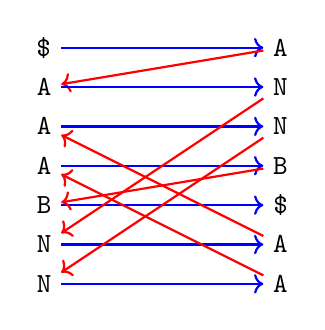
\begin{tikzpicture}
        % Horizontal distance = vertical height = 6 units
        \def\hsep{3}
        
        % Left column (top to bottom)
        \node (l1) at (0,3) {\texttt{\$}};
        \node (l2) at (0,2.5) {\texttt{A}};
        \node (l3) at (0,2) {\texttt{A}};
        \node (l4) at (0,1.5) {\texttt{A}};
        \node (l5) at (0,1) {\texttt{B}};
        \node (l6) at (0,.5) {\texttt{N}};
        \node (l7) at (0,0) {\texttt{N}};
        
        % Right column (top to bottom)
        \node (r1) at (\hsep,3) {\texttt{A}};
        \node (r2) at (\hsep,2.5) {\texttt{N}};
        \node (r3) at (\hsep,2) {\texttt{N}};
        \node (r4) at (\hsep,1.5) {\texttt{B}};
        \node (r5) at (\hsep,1) {\texttt{\$}};
        \node (r6) at (\hsep,.5) {\texttt{A}};
        \node (r7) at (\hsep,0) {\texttt{A}};
        \pause
        \draw[->, blue, thick] (l1) -- (r1);
        \pause 
        \draw[->, red, thick] (r1) -- (l2); % $ -> U
        \pause
        \draw[->, blue, thick] (l2) -- (r2); % 
        \pause
        % L-> R
        ; % 
        \draw[->, blue, thick] (l3) -- (r3); % 
        \draw[->, blue, thick] (l4) -- (r4); % 
        \draw[->, blue, thick] (l5) -- (r5); % 
        \draw[->, blue, thick] (l6) -- (r6); % 
        \draw[->, blue, thick] (l7) -- (r7); % 
        
        % Arrows from right to left (originally green, now blue)
        \draw[->, red, thick] (r2) -- (l6); % A -> V
        \draw[->, red, thick] (r3) -- (l7); % A -> $
        \draw[->, red, thick] (r4) -- (l5); % A -> B
        % \draw[->, red, thick] (r5) -- (l3); % B -> N
        \draw[->, red, thick] (r6) -- (l3); % N -> N
        \draw[->, red, thick] (r7) -- (l4); % N -> A

        \end{tikzpicture}
        \end{center}
    
        \pause
        \only<+->{\centering follow the tip of blue arrows to get back the initial message: \texttt{BANANA\$}}
    
\end{frame}

\begin{frame}{EXACTMATCH Algoritham}
    We have, $T=\texttt{B}_1\texttt{A}_1\texttt{N}_1\texttt{A}_2\texttt{N}_2\texttt{A}_3$.\\
    Pattern to find, $P = \texttt{NAN}$\\
    \begin{center}
        \begin{tikzpicture}
        % Horizontal distance = vertical height = 6 units
        \def\hsep{2}
        
        \node (l1) at (0,3) {\texttt{\$}};
        \node (l2) at (0,2.5) {\texttt{A}$_1$};
        \node (l3) at (0,2) {\texttt{A}$_2$};
        \node (l4) at (0,1.5) {\texttt{A}$_3$};
        \node (l5) at (0,1) {\texttt{B}$_1$};
        \node (l6) at (0,.5) {\texttt{N}$_1$};
        \node (l7) at (0,0) {\texttt{N}$_2$};
        % Right column (top to bottom)
        \node (r1) at (\hsep,3) {\texttt{A$_1$}};
        \node (r2) at (\hsep,2.5) {\texttt{N$_1$}};
        \node (r3) at (\hsep,2) {\texttt{N$_2$}};
        \node (r4) at (\hsep,1.5) {\texttt{B$_1$}};
        \node (r5) at (\hsep,1) {\texttt{\$}};
        \node (r6) at (\hsep,.5) {\texttt{A$_2$}};
        \node (r7) at (\hsep,0) {\texttt{A$_3$}};
        \pause
        %Indices:
        \node (il1) at (-1,3) {0};
        \node (il2) at (-1,2.5) {1};
        \node (il3) at (-1,2) {2};
        \node (il4) at (-1,1.5) {3};
        \node (il5) at (-1,1) {4};
        \node (il6) at (-1,.5) {5};
        \node (il7) at (-1,0) {6};

        %Right Indices
        \node (ir1) at (\hsep+1,3) {1};
        \node (ir2) at (\hsep+1,2.5) {5};
        \node (ir3) at (\hsep+1,2) {6};
        \node (ir4) at (\hsep+1,1.5) {4};
        \node (ir5) at (\hsep+1,1) {0};
        \node (ir6) at (\hsep+1,.5) {2};
        \node (ir7) at (\hsep+1,0) {3};
        \pause 
        \only<3>{\node[text=red] (top) at (-3, 3) {top$\rightarrow$};}
        \only<3>{\node[text=red] (bot) at (-3, 0) {bot$\rightarrow$};}

        \only<4>{\node[text=red] (top) at (-3, 0.5) {top \texttt{N$_1$}$\rightarrow$};}
        \only<4>{\node[text=red] (bot) at (-3, 0) {bot \texttt{N$_2$}$\rightarrow$};}

        \only<5>{\node[text=red] (top) at (-3, 2) {top \texttt{A$_2$N$_1$}$\rightarrow$};}
        \only<5>{\node[text=red] (bot) at (-3, 1.5) {bot \texttt{A$_3$N$_2$}$\rightarrow$};}
        
        \only<6>{\node[text=red] (top) at (-3, 0) {top/bot: \texttt{N$_2$A$_2$N$_1$}$\rightarrow$};}
        % \only<6>{\node[text=black] (bot) at (-3, 1) {\texttt{B$_1$A$_3$N$_2$}$\rightarrow$};}

    \end{tikzpicture}
    \end{center} 
\end{frame}

\section{Bowtie algorithm}
\begin{frame}{Exact vs Inexact Matching}
    \begin{itemize}
        \item EXACTMATCH algorithm is insufficient for DNA short read alignment.
        \item So, Bowtie algorithm follows a specified alignment policy:
        \begin{itemize}
    
        \item Each character in a read has a numeric quality value($m_i$), with
        lower values indicating a higher likelihood of a sequencing
        error. 
        \item We allows a limited number of mismatches, while trying to minimize $\sum_i m_i$, 
        where $i$ covers all the mismatches and performs a greedy search.  
        \end{itemize}
    \end{itemize} 
    \vspace{5mm}
    Bowtie is a quality-aware, greedy, randomized, depth-first search through the
    space of possible alignments.
\end{frame}

\begin{frame}{Excessive Backtracking}
    If a particular suffix doesn't occur in the 
    text, the algorithm can backtrack. Backtracking involves \textbf{potentially substituting 
    a different base at an already-matched query position, introducing a mismatch, and 
    then resuming the search.}\\
\vspace{5mm}
    Excessive backtracking occurs when too many alternative paths are explored during the alignment 
    process due to mismatches. Bowtie uses double indexing to deal with this problem.
    Excessive backtracking is significant only when a read has many low-quality 
    positions and does not align or aligns poorly to the reference.
\end{frame}

\begin{frame}{Mismatch Cases}
\begin{itemize}
    \item The high-quality base-pairs at 3' is called Seed(default: 28). 
    \item Seed is further divided into hi-half and lo-half each with 14bps.
    \item  Assuming the default mismatches(2), a reportable alignment can occur in 
    4 different ways. 
    \begin{enumerate}
        \item No mismatches in seed
        \item No mismatches in hi-half, one or two mismatches in lo-half
        \item No mismatches in lo-half, one or two mismatches in hi-half
        \item O ne mismatch in hi-half, one mismatch in lo-half
    \end{enumerate} 
\end{itemize}
\end{frame}

\begin{frame}{Phased Maq-like Search}
    Bowtie uses a 3 phase approach:
    \begin{columns}
        \begin{column}{.3\textwidth}
        \begin{figure}
            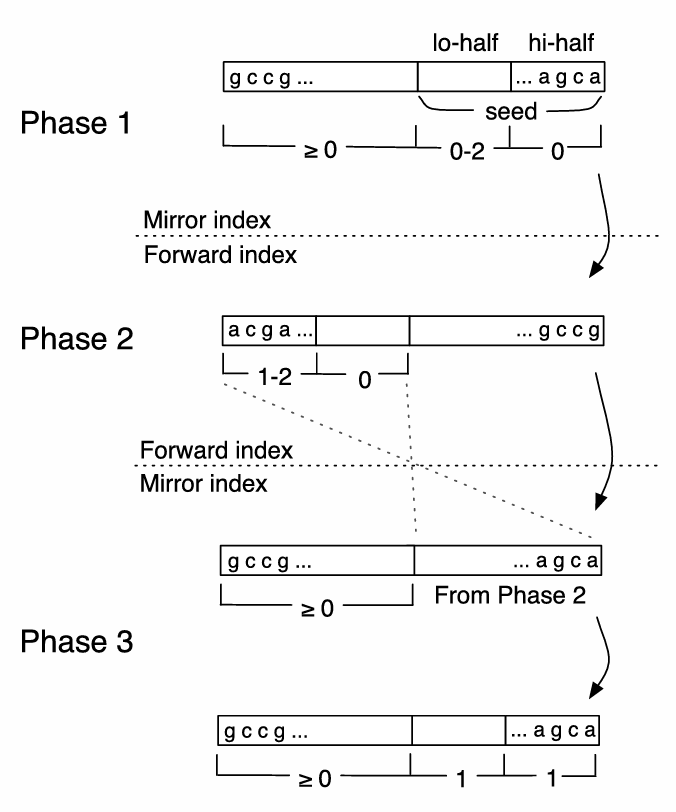
\includegraphics[scale=.25]{media/fig3.png}
        \end{figure}
        \end{column}
        \begin{column}{.7\textwidth}
            \begin{enumerate}
            \item Phase 1 uses the mirror index and invokes the
            aligner to find alignments for cases 1 and 2. 
            \item Phases 2 and 3 cooperate to find alignments for case 3. Phase 2 finds partial
            alignments with mismatches only in the hi-half and phase 3
            attempts to extend those partial alignments into full align
            ments. Finally, phase 3 invokes the aligner to find alignments
            for case 4.
            \end{enumerate}
        \end{column}
    \end{columns}
\end{frame}

\section{Results}

\begin{frame}{Summary of Results}
    \begin{itemize}
        \only<1>{\item \textbf{Speed:} Bowtie is significantly faster (\textit{Table 1}). When 
        aligning 8.84 million 35-bp reads to the human genome, Bowtie on a server 
        achieved 33.8 million reads/CPU hour, which is 351$\times$ faster than SOAP 
        (0.10 million reads/hour) and 107$\times$ faster than Maq (0.27 million 
        reads/hour).}
        \only<2>{\item \textbf{Memory:} For the human genome, its memory footprint is approximately 1.3 GB. 
        This small footprint allows Bowtie to run on a typical desktop computer with 2 GB 
        of RAM, something SOAP could not do.}
        \only<3>{\item \textbf{Sensitivity:} Bowtie's default sensitivity is comparable to SOAP's 
        ($\approx$67\%) and slightly less than Maq's (Bowtie 71.9\% vs Maq 74.7\% 
        in Table 1). The slight difference is mainly because Maq's algorithm is 
        more flexible, sometimes allowing three mismatches in the seed, and also 
        due to Bowtie's backtrack ceiling. Most of this can be manually fine-tuned.}
        \only<4>{\item \textbf{Read Length:} Maq scales better overall to longer reads than Bowtie or SOAP. However, 
        Bowtie in SOAP-like \texttt{-v 2} mode scales very well. Bowtie in its default 
        Maq-like mode is slower for 76-bp reads compared to shorter reads but still 
        significantly faster than Maq.}
        \only<5>{\item \textbf{Parallel Performance:} Bowtie supports parallel processing. 
        On a four-core server, using four threads provided a speedup of 3.12$\times$ compared 
        to single thread. The memory footprint doesn't increase substantially with more
        threads as the index is shared(\textit{Table 4}).}
        \only<6>{\item \textbf{Index Building:} Unlike tools that build index-systems during alignment, Bowtie 
        creates a permanent index that can be reused. 1
        Eventhough indexing the human genome takes hours, depending on the memory target, including 
        index construction time, Bowtie still outperforms competing tools when aligning large 
        datasets(\textit{Table 5})}
    \end{itemize}
\end{frame}


\begin{frame}{Perfomance Results}
\begin{center}        
    \begin{figure}
        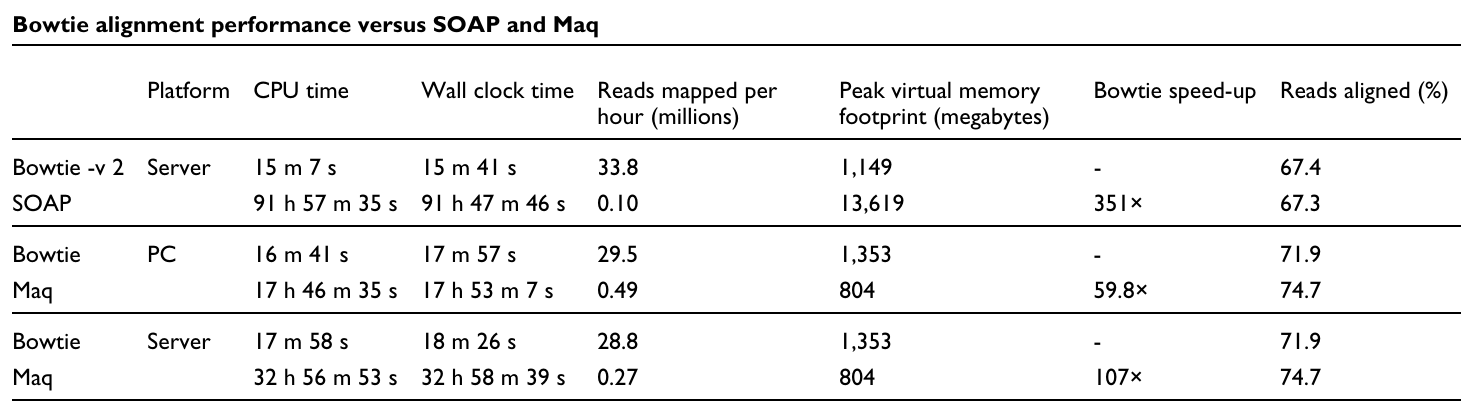
\includegraphics[width=\textwidth]{media/tab1.png}
    \end{figure} \tiny Table 1
    \pause
    \begin{figure}
        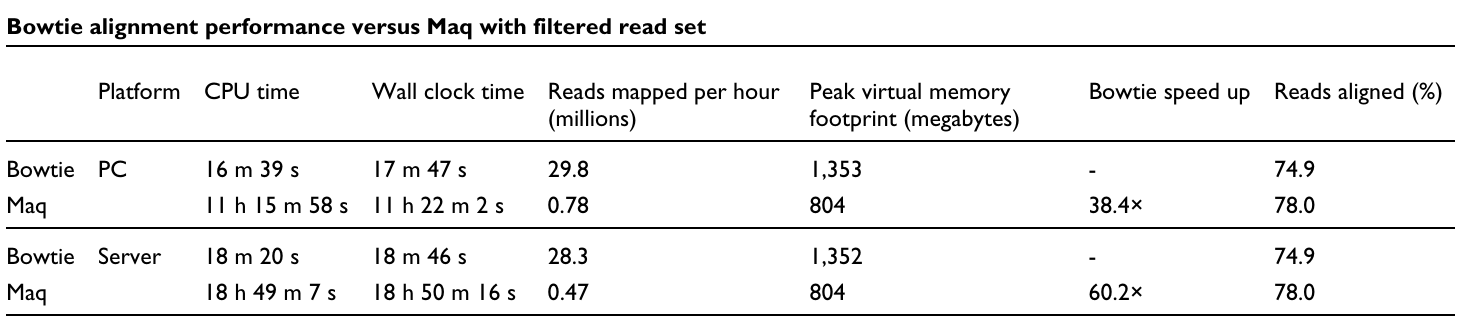
\includegraphics[width=\textwidth]{media/tab2.png}
    \end{figure}\tiny Table 2
\end{center}
\end{frame}

\begin{frame}{Perfomance Results-II}
    \begin{figure}
        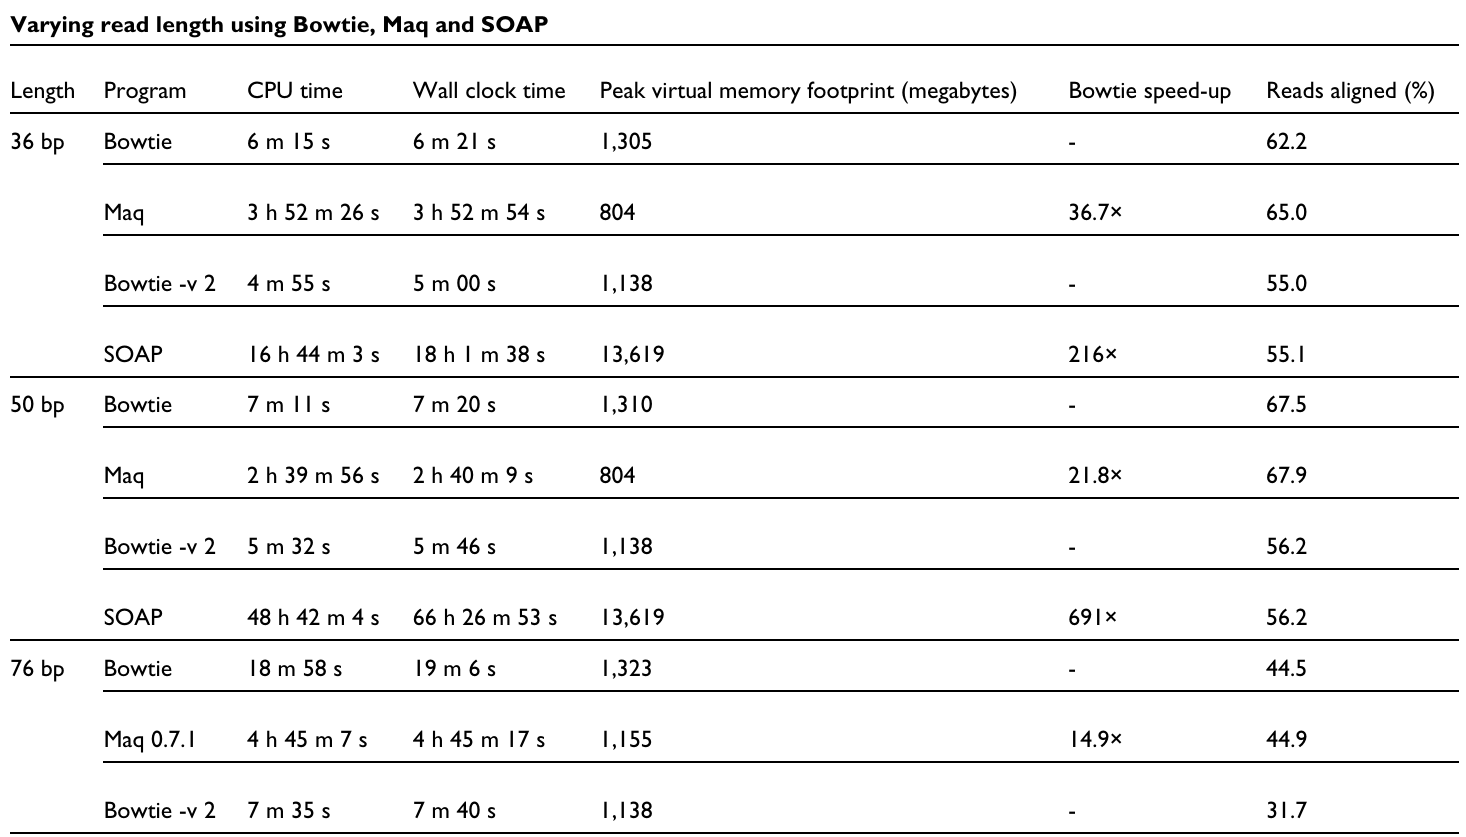
\includegraphics[width=\textwidth]{media/tab3.png}
    \end{figure}\centering \tiny Table 3
\end{frame}

\begin{frame}{Perfomance Results-III}
    \begin{figure}
        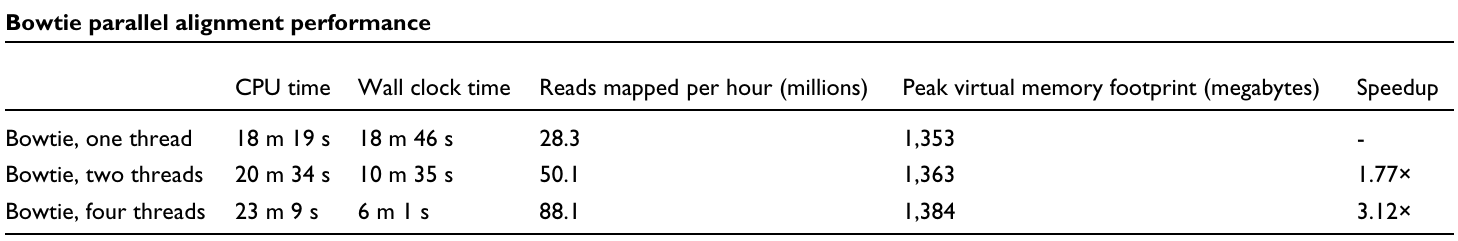
\includegraphics[width=\textwidth]{media/tab4.png}
    \end{figure}\centering \tiny Table 4
    \pause
    \begin{figure}
        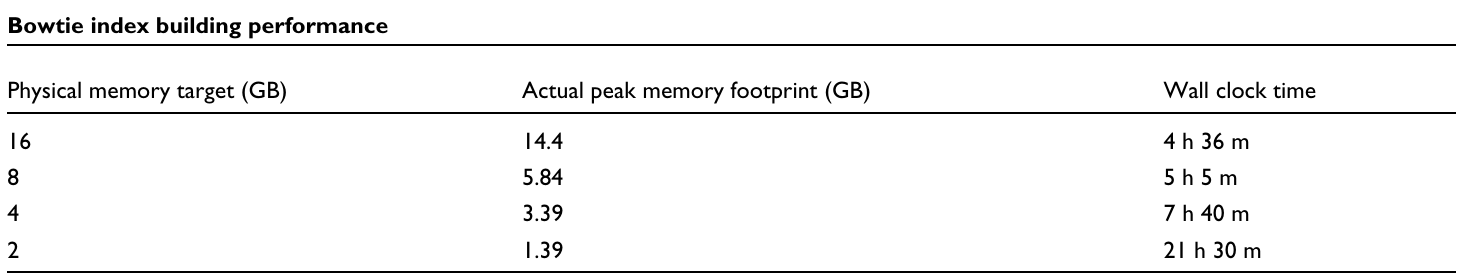
\includegraphics[width=\textwidth]{media/tab5.png}
    \end{figure} \centering \tiny Table 5
\end{frame}

\begin{frame}{Summary}
    \begin{itemize}
        \item Bowtie's speed and small memory footprint are due chiefly to
        its use of the Burrows-Wheeler index in combination with the
        novel, quality-aware, backtracking algorithm introduced
        here. Double indexing is used to avoid the performance penalty
        of excessive backtracking.
        \item Bowtie exhibits a large performance advantage over both Maq
        and SOAP when mapping reads to the human genome.
        \item  Unlike many other short-read aligners, Bowtie creates a per
        manent index of the reference that may be re-used across
        alignment runs. 
    \end{itemize}
\end{frame}

\begin{frame}{}
 \begin{center}
    \Huge Thank you!
 \end{center}
\end{frame}
\end{document}